\chapter{DASAR TEORI}
\par Bab ini menjelaskan dasar teori yang penulis gunakan sebagai landasan pengerjaan tugas akhir. Bab ini akan menjelaskan secara umum terkait istilah dan kakas bantu yang digunakan dalam pembuatan tugas akhir ini.

\section{Penelitian Sebelumnya}
\par Tugas akhir ini merupakan pengembangan dari penelitian "Rancang Bangun Aplikasi Push Notification Terpusat" \cite{application-thesis}. Penelitian tersebut menghasilkan aplikasi yang bernama Push Notification Terpusat.
\par Push Notification Terpusat merupakan aplikasi yang dibuat untuk memudahkan penyebaran informasi di lingkungan ITS sebagai pengganti media cetak. Aplikasi ini dapat mengirim notifikasi secara langsung atau terjadwal ke perangkat pengguna (Android dan iOS). Arsitektur aplikasi dapat dilihat pada Gambar \ref{img:arsitektur-pnt_lama}.
\begin{figure}[H]
	\centering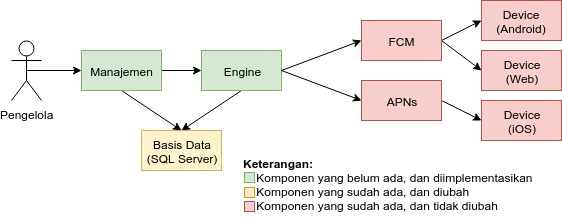
\includegraphics[width=1\textwidth]{bab2/img/arsitektur-push_notification_terpusat_lama.jpg}
	\caption{Arsitektur Push Notification Terpusat Saat Ini}
	\label{img:arsitektur-pnt_lama}
\end{figure}
\par Modul Manajemen bertanggung jawab untuk menangani interaksi pengelola dengan sistem lewat halaman web, sementara modul Engine bertanggung jawab untuk mengirimkan notifikasi ke layanan FCM dan APNs.
\par Proses pengiriman notifikasi dengan menggunakan Push Notification Terpusat adalah sebagai berikut:
\begin{enumerate}
	\item Pengelola mengakses halaman kirim notifikasi pada modul manajemen.
	\item Pengelola memasukkan data notifikasi, yaitu judul dan isi pesan, pengguna yang menerima notifikasi, dan aplikasi yang digunakan.
	\item Manajemen menyimpan data yang dimasukan pengguna sebagai \textit{batch} ke basis data.
	\item Manajemen mengirimkan permintaan pengiriman \textit{batch} ke Engine.
	\item Engine menambahkan \textit{batch} ke antrian.
	\item Engine mengambil data \textit{batch} dari antrian, dan dikirim ke layanan FCM atau APNs.
\end{enumerate}
\par Aplikasi yang dibuat pada penelitian sebelumnya sudah dapat digunakan untuk mengirim notifikasi, akan tetapi aplikasi masih memiliki kelemahan dari sisi keandalan pengiriman notifikasi, karena hanya mampu mengirim hingga 1.900 notifikasi dalam satu waktu. Hasil uji dapat dilihat pada Tabel \ref{t:hasil_uji_sebelum} \cite{application-thesis}.
\begin{longtable}{|p{1.5cm}|p{2cm}|p{2cm}|p{2.5cm}|}
	\caption{Hasil Uji Penelitian Sebelumnya} \label{t:hasil_uji_sebelum} \\ \hline
	\rowcolor{lightgray} Kode Uji & Jumlah Pengguna & Tingkat Keberhasilan & Rata-Rata \textit{Response Time} (detik) \\ \hline
	\endfirsthead
	\hline
	\rowcolor{lightgray} Kode Uji & Jumlah Pengguna & Tingkat Keberhasilan & Rata-Rata \textit{Response Time} (detik) \\ \hline
	\endhead
	RT001 & 100 & 100\% & 0,334 \\ \hline
	RT002 & 500 & 100\% & 2,326 \\ \hline
	RT003 & 1000 & 100\% & 4,664 \\ \hline
	RT004 & 2000 & 80,7\% & 8,889 \\ \hline
	RT005 & 3000 & 63,8\% & 10,552 \\ \hline
\end{longtable}
\par Berdasarkan hasil uji, dapat dikatakan bahwa aplikasi yang dibangun sebelumnya hanya dapat menangani sekitar 1.500 pengguna. Jumlah ini dianggap belum dapat memenuhi kebutuhan, karena target pengguna aplikasi ini adalah mahasiswa, dosen, dan karyawan yang ada di ITS.
\par Oleh karena itu, pengembangan yang dilakukan pada tugas akhir ini akan berfokus pada perbaikan modul Engine untuk meningkatkan keandalan pengiriman notifikasi.

\section{Apple Push Notification Service}
\par Apple Push Notification Service atau APNs adalah layanan pengiriman notifikasi jarak jauh yang kuat, cepat dan sangat efisien, yang dapat digunakan oleh pengembang aplikasi untuk menyebarkan informasi ke perangkat iOS, watchOS, tvOS, dan macOS. Ukuran maksimum notifikasi yang dapat dikirim adalah 4 Kb, dan wajib menggunakan protokol TLS, dengan alur yang dapat dilihat pada Gambar \ref{img:apns-certificate} \cite{apns-online}.
\begin{figure}[H]
	\centering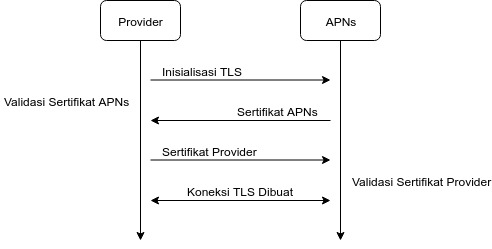
\includegraphics[width=1\textwidth]{bab2/img/activity-apns_certificate_connection.jpg}
	\caption{Alur Autentikasi APNs}
	\label{img:apns-certificate}
\end{figure}
\par Untuk dapat menerima dan mengontrol \textit{remote notification}, aplikasi harus memenuhi syarat sebagai berikut.
\begin{enumerate}
	\item Mengaktifkan kemampuan push notifications dengan cara memindah \textit{switch} posisi \textit{off} menjadi \textit{on} pada jendela \textit{Project editor} > \textit{Target} > \textit{Capabilities}.
	\item Melakukan registrasi aplikasi kepada APNs dengan cara menerima \textit{token} yang bersifat unik untuk tiap perangkat yang berbeda.
	\item Sistem akan menampilkan perangkat ke aplikasi Anda dengan memanggil metode di delegasi aplikasi. Aplikasi mengirimkan \textit{token} perangkat ke penyedia yang terkait dengan aplikasi.
\end{enumerate}
\par Contoh program yang digunakan untuk mengirim notifikasi ke perangkat iOS lewat layanan APNs dapat dilihat pada Kode Sumber \ref{json:contoh-apns}. Hasil notifikasi yang diterima oleh pengguna dapat dilihat pada Gambar \ref{img:contoh-hasil-apns}.
\par Pada tugas akhir ini, \textit{push notification} yang menargetkan perangkat iOS akan dikirim dengan menggunakan layanan Apple Push Notification Service.
\lstinputlisting[label=json:contoh-apns, caption={Contoh \textit{Push Notification} APNs}] {bab2/json/apns.json}
\begin{figure}[H]
	\centering
\includegraphics[width=0.8\textwidth]{bab2/img/apns.jpg}
	\caption{Pratinjau Notifikasi pada iOS}
	\label{img:contoh-hasil-apns}
\end{figure}

\section{Firebase Cloud Messaging}
\par Firebase Cloud Messaging atau FCM adalah solusi pengiriman pesan lintas \textit{platform} yang dapat diandalkan untuk mengirimkan pesan dan dapat digunakan tanpa biaya. FCM memiliki kemampuan sebagai berikut \cite{fcm-online}:
\begin{enumerate}[listparindent=2.5em]
	\item Mengirimkan notifikasi atau pesan data
	\par Mengirim pesan notifikasi yang ditampilkan kepada pengguna. Atau mengirim pesan data dan menentukan sepenuhnya apa yang terjadi dalam kode aplikasi.
	\item Penargetan pesan serbaguna
	\par Mendistribusikan pesan ke aplikasi klien dengan salah satu dari tiga cara, ke satu perangkat, ke grup perangkat, atau ke perangkat yang berlangganan topik.
	\item Mengirim pesan dari aplikasi \textit{client}
	\par Mengirim notifikasi, \textit{chat}, dan pesan lain dari perangkat ke \textit{server} melalui saluran koneksi FCM yang andal dan hemat baterai.
\end{enumerate}
\par Untuk mengimplementasikan FCM, pengembang harus mengikuti langkah-langkah berikut:
\begin{enumerate}[listparindent=2.5em]
	\item Menyiapkan FCM SDK
	\par Menyiapkan Firebase dan FCM pada aplikasi sesuai petunjuk penyiapan untuk \textit{platform} (Android atau Web).
	\item Mengembangkan aplikasi klien
	\par Menambahkan penanganan pesan, logika langganan topik, atau fitur opsional lain ke aplikasi \textit{client}. Selama pengembangan, dapat dilakukan pengujian untuk mengirim pesan dengan mudah menggunakan \textit{Firebase Console}.
	\item Mengembangkan \textit{server} aplikasi
	\par Tentukan apakah pengembangan nantinya menggunakan Admin SDK atau salah satu \textit{server} \textit{protocol} untuk membuat logika pengiriman, yaitu logika untuk mengautentikasi, membuat permintaan pengiriman, menangani respons, dan sebagainya.
\end{enumerate}
\par Contoh program yang digunakan untuk mengirim notifikasi ke perangkat Android lewat layanan FCM dapat dilihat pada Kode Sumber \ref{json:contoh-fcm}. Hasil notifikasi yang diterima oleh pengguna dapat dilihat pada Gambar \ref{img:contoh-hasil-fcm}.
\par Pada tugas akhir ini, \textit{push notification} yang menargetkan perangkat Android dan Web akan dikirim ke layanan FCM oleh Push Notification Terpusat.
\lstinputlisting[label=json:contoh-fcm, caption={Contoh \textit{Push Notification} FCM}] {bab2/json/fcm.json}
\begin{figure}[H]
	\centering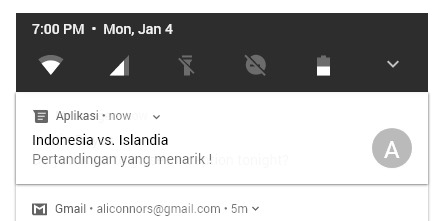
\includegraphics[width=0.8\textwidth]{bab2/img/fcm.jpg}
	\caption{Pratinjau Notifikasi pada Android}
	\label{img:contoh-hasil-fcm}
\end{figure}

\section{Microsoft SQL Server}
\par Microsoft SQL Server atau SQL Server adalah sebuah sistem manajemen basis data relasional (RDBMS) yang merupakan produk dari Microsoft. Bahasa \textit{query} utamanya adalah Transact-SQL yang merupakan implementasi dari SQL standar ANSI/ISO yang digunakan oleh Microsoft dan Sybase. SQL Server banyak digunakan pada dunia bisnis, pendidikan, dan juga pemerintahan sebagai solusi penyimpanan data \cite{sql-server-online}.
\par SQL Server dan Sybase/ASE dapat berkomunikasi lewat jaringan menggunakan protokol TDS (\textit{Tabular Data Stream}). Selain itu, SQL Server juga mendukung ODBC (\textit{Open Database Connectivity}) dan mempunyai \textit{driver} JDBC untuk bahasa pemrograman Java. Fitur lain dari SQL Server yaitu kemampuannya untuk membuat basis data \textit{mirroring} dan \textit{clustering}.
\par Pada tugas akhir ini, SQL Server akan digunakan untuk penyimpanan dan pencarian data yang dibutuhkan oleh Push Notification Terpusat.

\section{Antrian Pesan}
\par Antrian pesan atau \textit{message queue} adalah metode komunikasi untuk pertukaran pesan antar sistem, dengan cara menyediakan media penyimpanan pesan sementara ketika sistem yang dituju sedang sibuk.
\par Arsitektur antrian pesan terdiri dari \textit{producer} yang membuat dan mengirim pesan ke antrian, dan \textit{consumer} yang mengambil dan mengolah pesan dari antrian. Arsitektur antrian pesan dapat dilihat pada Gambar \ref{img:arsitektur-mq_pnt} \cite{message-queue-online}.
\begin{figure}[H]
	\centering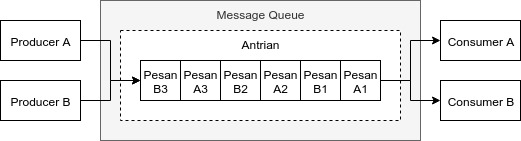
\includegraphics[width=1\textwidth]{bab2/img/arsitektur-mq_pnt.jpg}
	\caption{Arsitektur Antrian Pesan}
	\label{img:arsitektur-mq_pnt}
\end{figure}
\par Pada tugas akhir ini, antrian pesan merupakan metode yang digunakan untuk menangani pengiriman \textit{push notification}. Perbandingan tanpa dan dengan antrian pesan dapat dilihat pada Tabel \ref{t:perbandingan-antrian-pesan}.
\begin{longtable}{|p{4.5cm}|p{4.5cm}|}
	\caption{Perbandingan Penggunaan Antrian Pesan} \label{t:perbandingan-antrian-pesan} \\ \hline
	\rowcolor{lightgray} Tanpa Antrian Pesan & Dengan Antrian Pesan \\ \hline
	\endfirsthead
	\hline
	\rowcolor{lightgray} Tanpa Antrian Pesan & Dengan Antrian Pesan \\ \hline
	\endhead
	\textit{Client} dapat melihat langsung hasil \textit{request}. & \textit{Client} hanya mengetahui jika \textit{request} sudah tersimpan dan akan dijalankan. \\ \hline
	Jika \textit{request} gagal, \textit{client} bertanggung jawab untuk mengulang operasi. & Jika \textit{request} gagal, \textit{server} bertanggung jawab untuk mengulang operasi. \\ \hline
	Spesifikasi sistem harus mencukupi penggunaan sumber daya. & Penggunaan sumber daya dapat menyesuaikan spesifikasi sistem. \\ \hline
\end{longtable}

\section{Apache Kafka}
\par Apache Kafka atau Kafka adalah layanan terdistribusi untuk data \textit{streaming} \cite{kafka-online}. Kafka pada dasarnya merupakan pengembangan dari arsitektur antrian pesan, dimana terdapat \textit{producer} dan \textit{consumer} yang memproduksi dan mengambil pesan dari dan ke antrian. Perbedaannya, Kafka membagi antrian berdasarkan topik dan partisi.
\begin{figure}[H]
	\centering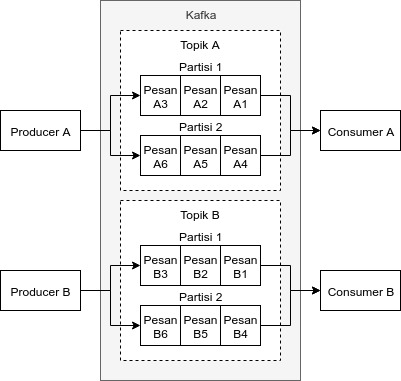
\includegraphics[width=1\textwidth]{bab2/img/arsitektur-mq_kafka.jpg}
	\caption{Arsitektur Antrian Pesan Apache Kafka}
	\label{img:arsitektur-mq_kafka}
\end{figure}
\par \textit{Producer} dan \textit{consumer} pada Kafka dapat memilih antrian mana yang ingin digunakan berdasarkan nama topik. Pengguna juga dapat mengkonfigurasi nilai partisi suatu antrian, pesan yang berada dalam satu partisi akan diolah secara terurut (\textit{synchronous}), dan yang berbeda partisi akan diolah secara bersamaan (\textit{asynchronous}). Gambar arsitektur antrian dapat dilihat pada Gambar \ref{img:arsitektur-mq_kafka} \cite{kafka-online}.
\par Untuk menjalankan Kafka, pengembang perlu menjalankan Apache Zookeeper terlebih dahulu. Apache Zookeeper atau Zookeeper merupakan aplikasi yang digunakan oleh Kafka untuk mengatur sinkronisasi \textit{producer}, \textit{consumer}, dengan topik dan partisi antrian.
\par Pada tugas akhir ini, Kafka akan digunakan sebagai pengganti antrian pesan Push Notification Terpusat. Tabel perbandingan antrian pesan Push Notification Terpusat dengan Apache Kafka dapat dilihat pada Tabel \ref{t:perbandingan_kafka}.
\begin{longtable}{|p{2.5cm}|p{3.5cm}|p{3.5cm}|}
	\caption{Perbandingan Antrian Pesan Push Notification Terpusat dengan Apache Kafka} \label{t:perbandingan_kafka} \\ \hline
	\rowcolor{lightgray} Kategori & Push Notification Terpusat & Apache Kafka \\ \hline
	\endfirsthead
	\hline
	\rowcolor{lightgray} Kategori & Push Notification Terpusat & Apache Kafka \\ \hline
	\endhead
	Penyimpanan pesan & \textit{Non Persistence}, disimpan dalam sistem, akan hilang jika sistem mati. & \textit{Persistence}, disimpan dalam media penyimpanan perangkat, tetap tersimpan meskipun sistem mati. \\ \hline
	Jumlah pesan maksimum & Dapat menangani 1.000 pesan tanpa gagal. & Dapat menangani 1.000.000 pesan tanpa gagal. \\ \hline
	Arsitektur antrian & Satu antrian untuk semua pesan. & Antrian dibagi berdasarkan topik dan partisi. \\ \hline
	Urutan pengambilan pesan & Terurut berdasarkan waktu ditambahkan. & Jika di satu partisi, terurut berdasarkan waktu ditambahkan. Jika berbeda partisi, berdasarkan partisi manapun yang tidak kosong. \\ \hline
\end{longtable}

% \section{Apache Zookeeper}
% \par Apache Zookeeper atau Zookeeper adalah layanan koordinasi untuk aplikasi terdistribusi. Zookeeper mengatur hal-hal umum dalam aplikasi terdistribusi, seperti penamaan, konfigurasi, sinkronisasi, dan pengelompokan layanan \cite{zookeeper-online}.
% \par Pada tugas akhir ini, Zookeeper merupakan layanan yang dibutuhkan oleh Kafka untuk beroperasi. Kafka menggunakan Zookeeper untuk mengatur koordinasi \textit{producer} dan \textit{consumer} dengan antrian pesan.

\section{Java}
\par Java adalah bahasa pemrograman yang umum, konkuren, berbasis kelas, dan berbasis objek \cite{java-online}. Beberapa fitur Java yang akan digunakan dalam implementasi tugas akhir ini adalah sebagai berikut:
\begin{enumerate}[listparindent=2.5em]
	\item Lambda
	\par Lambda adalah ekspresi untuk inisiasi \textit{interface} fungsional (kelas \textit{interface} dengan satu fungsi abstrak). Lambda digunakan untuk implementasi fungsi tanpa harus membuat kelas, yang dapat diperlakukan seperti objek.
	\par Penulisan lambda diawali dengan parameter fungsi yang dibungkus dengan tanda kurung, karakter '->', dan implementasi fungsi yang dibungkus dengan kurung kurawal. Contoh implementasi lambda dapat dilihat pada Kode Sumber \ref{java:lambda}.
	\item Anotasi
	\par Anotasi adalah penanda untuk memberikan informasi tambahan tentang program. Beberapa contoh penggunaan anotasi adalah untuk dokumentasi program, memberi informasi \textit{error} ke \textit{compiler}, serialisasi data, dan \textit{mapping} kelas dengan basis data. 
	\par Penulisan anotasi diawali dengan karakter '@', nama anotasi, dan pasangan nama-nilai yang dibungkus dengan tanda kurung. Contoh implementasi anotasi dapat dilihat pada Kode Sumber \ref{java:annotation}.
\end{enumerate}
\lstinputlisting[label=java:lambda, caption=Contoh Implementasi Lambda pada Java, language=Java] {bab2/java/lambda.java}
\lstinputlisting[label=java:annotation, caption=Contoh Implementasi Anotasi pada Java, language=Java] {bab2/java/annotation.java}

\section{Spring}
\par Spring adalah kerangka kerja yang menyediakan dukungan infrastruktur lengkap untuk mengembangkan aplikasi Java \cite{spring-online}. Beberapa fitur Spring yang akan digunakan dalam implementasi tugas akhir ini adalah sebagai berikut:
\begin{enumerate}[listparindent=2.5em]
	\item \textit{Dependency Injection}
	\par \textit{Dependency injection} atau DI adalah proses untuk mendefinisikan objek dan dependensinya (objek lain yang dibutuhkan oleh objek tersebut). DI digunakan untuk memisahkan proses inisiasi objek dari proses bisnis, sehingga baris kode menjadi lebih rapih.
	\par Pada kerangka kerja Spring, implementasi DI adalah dengan menambahkan objek yang dibutuhkan ke \textit{constructor} atau \textit{setter} kelas. Contoh implementasi dapat dilihat pada Kode Sumber \ref{java:di-constructor}.
	\item \textit{Scheduling}
	\par \textit{Scheduling} adalah proses untuk mendefinisikan kapan sebuah fungsi akan dijalankan secara periodik. \textit{Scheduling} digunakan untuk proses-proses yang dilakukan berulang kali.
	\par Pada kerangka kerja Spring, implementasi \textit{scheduling} adalah dengan menambahkan anotasi @Scheduled di sebuah fungsi, dengan parameter berapa lama waktu yang dibutuhkan untuk menjalankan fungsi tersebut kembali. Contoh implementasi dapat dilihat pada Kode Sumber \ref{java:scheduling}.
\end{enumerate}
\lstinputlisting[label=java:di-constructor, caption=Contoh Implementasi \textit{Dependency Injection} pada Spring, language=Java] {bab2/java/di-constructor.java}
\lstinputlisting[label=java:scheduling, caption=Contoh Implementasi \textit{Scheduling} pada Spring, language=Java] {bab2/java/scheduling.java}
% DI, @Component, @Service, @Transactional, @Scheduled, @Cacheable, @KafkaListeners, Actuator

\section{Actuator}
\par Actuator berisi sekumpulan fitur tambahan untuk pemantauan dan pengaturan aplikasi yang sudah di tahap \textit{production}. Aplikasi bisa dipantau dan diatur dengan menggunakan \textit{endpoint} HTTP atau JMX \cite{actuator-online}.
\par Pada tugas akhir ini, Actuator merupakan pustaka yang digunakan dalam implementasi pemantauan Push Notification Terpusat. Fitur-fitur Actuator yang akan digunakan pada Push Notification Terpusat adalah sebagai berkut:
\begin{enumerate}[listparindent=2.5em]
	\item \textit{Metrics}
	\par Untuk menampilkan metrik yang berhubungan dengan sumber daya sistem yang terpakai, seperti CPU dan Memori.
	\item \textit{Health}
	\par Untuk menampilkan status kesehatan aplikasi, dan layanan-layanan yang berhubungan dengan aplikasi, seperti sistem basis data dan sistem antrian pesan.
	\item \textit{Environment}
	\par Untuk menampilkan konfigurasi Spring dan lingkungan sistem.
	\item \textit{Logfile}
	\par Untuk menampilkan \textit{log} yang dikeluarkan oleh sistem.
\end{enumerate}

\section{JSON}
\par JSON adalah format pertukaran data yang ringan, berbasis teks, dan independen. Nilai pada JSON dapat berupa \textit{object}, \textit{array}, \textit{number}, \textit{string}, \textit{true}, \textit{false}, atau \textit{null} \cite{json-online}. Struktur yang digunakan JSON untuk mengekspresikan nilai adalah sebagai berikut:
\begin{enumerate}[listparindent=2.5em]
	\item \textit{Object}
	\par Struktur \textit{object} direpresentasikan sebagai pasangan kurung kurawal, berisi beberapa pasangan nama dan nilai. Alur struktur \textit{object} dapat dilihat pada Gambar \ref{img:json-object}.
	\begin{figure}[H]
		\centering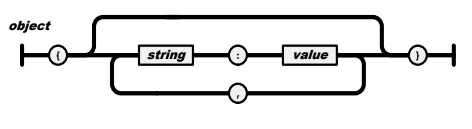
\includegraphics[width=0.9\textwidth]{bab2/img/json_object.jpg}
		\caption{Struktur JSON \textit{Object}} \label{img:json-object}
	\end{figure}
	\item \textit{Array}
	\par Struktur \textit{array} direpresentasikan sebagai pasangan kurung siku, berisi beberapa nilai, yang dipisahkan dengan koma. Alur struktur \textit{array} dapat dilihat pada Gambar \ref{img:json-array}.
	\begin{figure}[H]
		\centering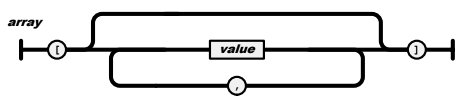
\includegraphics[width=0.9\textwidth]{bab2/img/json_array.jpg}
		\caption{Struktur JSON \textit{Array}} \label{img:json-array}
	\end{figure}
	\item \textit{Number}
	\par Struktur \textit{number} terdiri dari urutan bilangan desimal tanpa nol didepan. Nilai dapat memiliki tanda - dan + didepan, dan bagian pecahan diawali dengan titik. Bilangan yang tidak bisa direpresentasikan sebagai bilangan desimal, seperti \textit{infinity} dan \textit{NaN}, tidak diizinkan. Alur struktur \textit{number} dapat dilihat pada Gambar \ref{img:json-number}.
	\clearpage
	\begin{figure}[H]
		\centering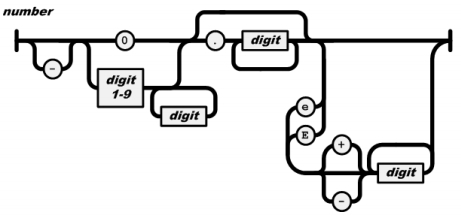
\includegraphics[width=0.9\textwidth]{bab2/img/json_number.jpg}
		\caption{Struktur JSON \textit{Number}} \label{img:json-number}
	\end{figure}
	\item \textit{String}
	\par Struktur \textit{string} direpresentasikan sebagai urutan karakter \textit{unicode} yang dibungkus dengan tanda kutip. Terdapat beberapa karakter yang harus di \textit{escape} agar dapat digunakan, yaitu:
	\begin{enumerate}
		\item \textbackslash " untuk karakter " (U+0022).
		\item \textbackslash\textbackslash\space untuk karakter \textbackslash\space (U+005C).
		\item \textbackslash / untuk karakter / (U+002F).
		\item \textbackslash b untuk karakter \textit{backspace} (U+0008).
		\item \textbackslash f untuk karakter \textit{form feed} (U+000C).
		\item \textbackslash n untuk karakter \textit{line feed} (U+000A).
		\item \textbackslash r untuk karakter \textit{return} (U+000D).
		\item \textbackslash t untuk karakter tabulasi (U+0009).
	\end{enumerate}
    \par Alur struktur \textit{string} dapat dilihat pada Gambar \ref{img:json-string}.
    \clearpage
    \begin{figure}[H]
    	\centering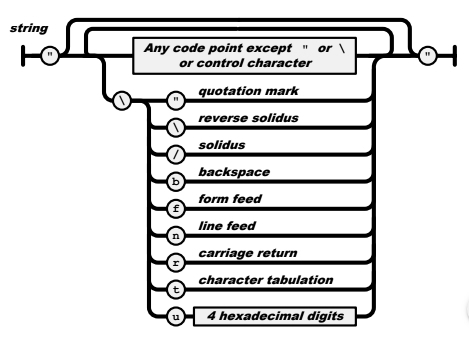
\includegraphics[width=0.9\textwidth]{bab2/img/json_string.jpg}
    	\caption{Struktur JSON \textit{String}} \label{img:json-string}
    \end{figure}
\end{enumerate}
\par Pada tugas akhir ini, JSON merupakan format pertukaran data yang digunakan oleh Kafka untuk menyimpan data, dan pustaka Actuator untuk menampilkan \textit{response}.

\section{Docker}
\par Docker adalah \textit{platform} terbuka untuk membangun, mengirim, dan menjalankan aplikasi. Docker memungkinkan pengembang untuk memisahkan kebutuhan infrastruktur dari aplikasi, sehingga proses pengembangan aplikasi bisa lebih cepat \cite{docker-online}.
\par Pada tugas akhir ini, Docker akan digunakan untuk menjalankan Push Notification Terpusat, Kafka, dan Zookeeper. Perbandingan penggunaan Docker dapat dilihat pada Tabel \ref{t:perbandingan_docker}, dan arsitektur Docker pada Gambar \ref{img:arsitektur-docker}.
\begin{longtable}{|p{2.5cm}|p{3.5cm}|p{3.5cm}|}
	\caption{Perbandingan Penggunaan Docker} \label{t:perbandingan_docker} \\ \hline
	\rowcolor{lightgray} Kategori & Tanpa Docker & Dengan Docker \\ \hline
	\endfirsthead
	\hline
	\rowcolor{lightgray} Kategori & Tanpa Docker & Dengan Docker \\ \hline
	\endhead
	Proses \textit{deployment} & Membutuhkan konfigurasi khusus untuk setiap sistem operasi & Dapat langsung dijalankan di sistem operasi manapun \\ \hline
	Pembatasan sumber daya & Tidak terbatas & Penggunaan CPU dan Memori bisa dibatasi \\ \hline
\end{longtable}
\begin{figure}[H]
\centering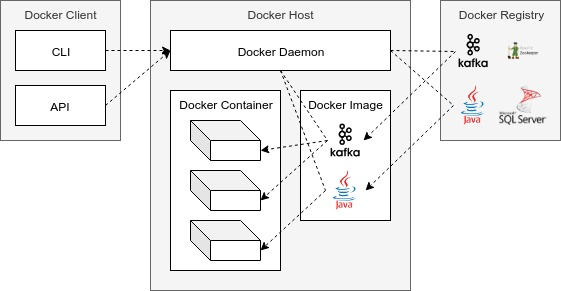
\includegraphics[width=0.9\textwidth]{bab2/img/arsitektur-docker.jpg}
\caption{Arsitektur Docker}
\label{img:arsitektur-docker}
\end{figure}

\section{Docker Compose}
\par Docker Compose adalah alat untuk mendefinisikan dan menjalankan beberapa \textit{container} aplikasi menggunakan Docker. Dengan Docker Compose, pengembang bisa menggunakan file berbasis YAML untuk mengatur konfigurasi layanan aplikasi, dan menggunakannya untuk membuat dan menjalankan layanan aplikasi \cite{docker-compose-online}.
\par Pada tugas akhir ini, Docker Compose akan digunakan untuk mendefinisikan konfigurasi yang digunakan untuk menjalankan Push Notification Terpusat, Kafka, dan Zookeeper. Perbandingan penggunaan Docker Compose dapat dilihat pada Tabel \ref{t:perbandingan_docker_compose}.
\begin{longtable}{|p{2cm}|p{3.5cm}|p{3.5cm}|}
	\caption{Perbandingan Penggunaan Docker Compose} \label{t:perbandingan_docker_compose} \\ \hline
	\rowcolor{lightgray} Kategori & Tanpa Compose & Dengan Compose \\ \hline
	\endfirsthead
	\hline
	\rowcolor{lightgray} Kategori & Tanpa Compose & Dengan Compose \\ \hline
	\endhead
	Konfigurasi & Ditambahkan dalam opsi setiap kali menjalankan \textit{container} & Disimpan dalam file \\ \hline
	Cara menjalankan & Untuk setiap \textit{container}, jalankan perintah "docker run <image>" untuk menjalankan \textit{container} & Jalankan perintah "docker-compose up" untuk menjalankan semua \textit{container} \\ \hline
\end{longtable}

\section{YAML}
\par YAML adalah bahasa untuk serialisasi data yang dirancang agar mudah dipahami oleh manusia dan bisa berjalan dengan bahasa pemrograman modern \cite{yaml-online}. Nilai pada YAML dapat berupa \textit{scalar}, \textit{sequence}, dan \textit{mapping}. Struktur yang digunakan YAML untuk mengekspresikan nilai adalah sebagai berikut:
\begin{enumerate}[listparindent=2.5em]
	\item \textit{Scalar}
	\par \textit{Scalar} adalah struktur digunakan untuk merepresentasikan sebuah teks atau bilangan. Nilai \textit{scalar} bisa saja dibungkus dengan tanda petik, namun tidak diwajibkan. Contoh \textit{scalar} dapat dilihat pada Kode Sumber \ref{yaml:scalar}.
	\item \textit{Sequence}
	\par \textit{Sequence} adalah struktur yang digunakan untuk merepresentasikan kumpulan nilai yang dipisah dengan karakter \textit{dash} (-). Contoh \textit{sequence} dapat dilihat pada Kode Sumber \ref{yaml:sequence}.
	\item \textit{Mapping}
	\par \textit{Mapping} adalah struktur yang digunakan untuk merepresentasikan kumpulan nilai dalam bentuk pasangan nama dan nilai. Contoh \textit{mapping} dapat dilihat pada Kode Sumber \ref{yaml:mapping}.
\end{enumerate}
\par Pada tugas akhir ini, YAML merupakan bahasa yang digunakan oleh Spring dan Docker Compose untuk mendefinisikan konfigurasi yang digunakan untuk menjalankan aplikasi.
\lstinputlisting[label=yaml:scalar, caption=Contoh Nilai \textit{Scalar} pada YAML] {bab2/yaml/yaml_scalar.yml}
\lstinputlisting[label=yaml:sequence, caption=Contoh Nilai \textit{Sequence} pada YAML] {bab2/yaml/yaml_sequence.yml}
\lstinputlisting[label=yaml:mapping, caption=Contoh Nilai \textit{Mapping} pada YAML] {bab2/yaml/yaml_mapping.yml}
